\section{Objectives and specification mapping}
Lab 7 (PDF pages 26--30) requires three tests: ring-oscillator stage counts N=3, 5 and 7 at fixed body bias; four body-bias configurations at fixed stage count; and NMOS/PMOS threshold versus reverse source-body bias. Both netlists and all five cases completed. Each oscillator case contains all three stage counts in parallel.

\section{Circuit and theory}
Each inverter has $W_n=0.6\,\mu$m, $W_p=1.8\,\mu$m and $L=0.25\,\mu$m. The final inverter feeds the first to form an odd-stage loop; no external oscillation clock is applied. UIC and a 0.05 V initial condition at one node break exact numerical symmetry. This is a transient-startup method, not a verification of undisturbed physical startup.

For average stage delay $t_p$, $T\approx2Nt_p$ and $f\approx1/(2Nt_p)$. The four cases are nominal bodies at 1 V/0 V; PMOS body at 1.2 V only; NMOS body at -0.2 V only; and both changes. The handout's 0.5 V offset at 2.5 V is scaled proportionally to 0.2 V at 1 V.

The long-channel NMOS body-effect relation is
\[V_{tn}=V_{tn0}+\gamma\left(\sqrt{2\phi_F+V_{SB}}-\sqrt{2\phi_F}\right).\]
PMOS uses the corresponding reverse bias and threshold magnitude. Short-channel, drain-bias and other effects remain in the simulator model; inaccessible $\gamma$ or $\phi_F$ coefficients are not invented.

\section{Simulation setup and measurement definitions}
The separately supplied MOS model is evaluated at 1.0 V and $27\,^{\circ}$C, retaining the handout topology and the comparison conditions below. One volt is a simulation setting, not a device rating established by available model documentation. Numerical results from the handout's older processes are not acceptance targets for this model.

HSPICE S-2021.09 runs with RUNLVL=6. Tables use actual native measurements and figures use actual printed numerical traces. Every variant resets all swept parameters and temperature, avoiding inherited settings from an earlier variant. Completed solutions and measurements do not establish process reliability. Internal warnings in encrypted model blocks remain incompletely visible.
Oscillator transients run for 20 ns with 1 ps printing. After discarding the first 10 ns, the first-to-sixth rising 50\% crossings span five periods, giving $f=5/\Delta t$. A separate DC source sweep covers 0--1 V in 10 mV increments and prints VTH directly rather than using an arbitrary current-threshold extraction.

\section{Measured results}
Frequencies below are in GHz and use actual settled threshold-crossing times.

\begin{center}\small
\begin{tabular}{llll}
\toprule
Body configuration & N=3 & N=5 & N=7 \\
\midrule
Nominal & 2.0095 & 1.1609 & 0.8279 \\
PMOS reverse bias & 1.9266 & 1.1101 & 0.7916 \\
NMOS reverse bias & 1.8870 & 1.0955 & 0.7814 \\
Dual reverse bias & 1.8112 & 1.0493 & 0.7485 \\
\bottomrule
\end{tabular}
\end{center}
\begin{figure}[htbp]
\centering
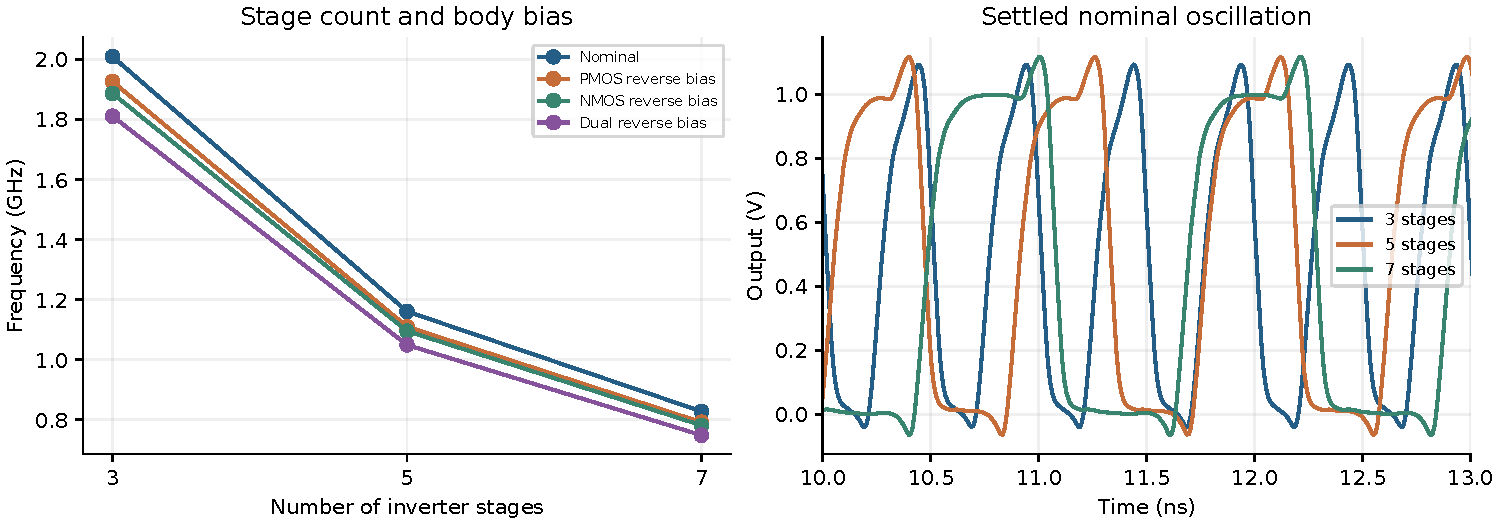
\includegraphics[width=\linewidth]{figures/ring_body_bias.pdf}
\caption{Stage count, reverse body bias, frequency and nominal oscillation waveforms.}
\end{figure}
\begin{center}\small
\begin{tabular}{llll}
\toprule
Device & Bias=0 V & Bias=1 V & Change (mV) \\
\midrule
NMOS & 0.3951 & 0.5804 & 185.29 \\
PMOS magnitude & 0.3364 & 0.5028 & 166.43 \\
\bottomrule
\end{tabular}
\end{center}
\begin{figure}[htbp]
\centering
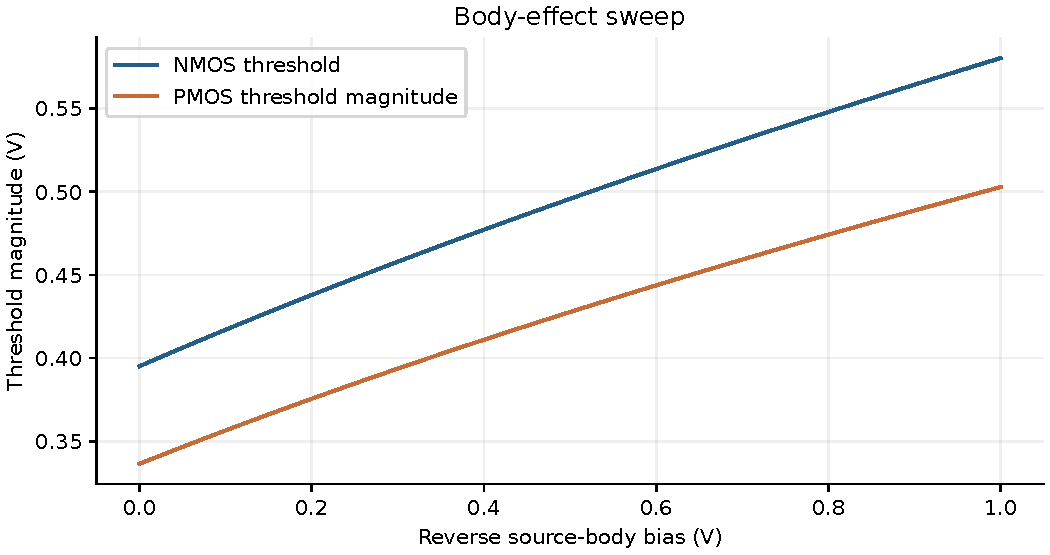
\includegraphics[width=.82\linewidth]{figures/body_threshold.pdf}
\caption{Direct VTH output shows increasing threshold magnitude for both device types under reverse bias.}
\end{figure}
\section{Discussion}
Increasing N increases loop delay and reduces frequency. Nominal inferred average stage delays are approximately 82.94/86.14/86.28 ps for N=3/5/7. The three-stage waveform and dynamic operating points differ, so identical $t_p$ for every N should not be assumed.

Reverse body bias raises threshold magnitude, reduces available overdrive and lowers frequency. The measured order is nominal, PMOS-only bias, NMOS-only bias and dual bias, matching the handout example. The relative effect of single-sided PMOS versus NMOS bias nevertheless depends on model and sizing; carrier mobility alone cannot establish that ranking for every process.

The plots retain small simulated overshoot and undershoot rather than clipping them to ideal 0/1 V levels. These traces do not establish reliability or junction-current compliance. The direct VTH sweep also includes other model bias effects and is not presented as an isolated extraction of long-channel body-effect coefficients.

\section{Reproducibility files}
The following netlists accompany this report. A comment marks the local model setup; neither the model file nor its path is published. A valid local model configuration must be supplied before execution.
\begin{itemize}
\item \texttt{01\_ring\_oscillators.sp}
\item \texttt{02\_body\_threshold.sp}
\end{itemize}
The lab results directory contains every case measurement, representative waveform CSV files, derived metrics and a specification manifest. Waveform exports retain at most 2501 uniformly selected samples; direct measurements are not downsampled. Complete original listings remain local.

